\documentclass[10pt,letterpaper,xcolor=dvipsnames,handout]{beamer}

%\usepackage[colorlinks=true,linkcolor=blue]{hyperref}
\usepackage{amssymb,mathabx}
\usepackage{linguex}
\usepackage{verbatim,enumerate,multirow}
\usepackage{xcolor}
%\usepackage{floatflt}

\include{beamer-ru101f14}

\AtBeginSubsection[]
{
     \begin{frame}<beamer>
       \frametitle{Lecture plan}
       \tableofcontents[currentsection,currentsubsection]
   \end{frame}
}

%For diagrams
\usepackage{tikz}
\usetikzlibrary{shapes,backgrounds}
\include{tikz-venn-diagrams}

\title{Categorical logic}
\subtitle{assessing inferences}
\author[Hoversten]{Erik Hoversten}
\institute[lrp-f14]{Logic, reason, and persuasion: fall 2014 \\ Rutgers University}
\date[10/02/2014]{October 2, 2014}

\begin{document}

\begin{frame}
\titlepage
\end{frame}

\section{Categorical logic}
\subsection{The language}

\begin{frame}
  \frametitle{Structure}
  
  We can think of logical systems as being defined by the \textbf{language} we use to express them.  Logical languages are similar to natural languages (English, Navajo) though they tend to be more constrained in what they can say.
  
  
  \begin{block}{Vocabulary}
    \begin{itemize}
      \item<2-> Logical:
        \begin{itemize}
          \item Quantifiers: \textit{all, some, no, some not}
          \item Copula: \textit{is, are, is not, are not}
        \end{itemize}
      \item<3-> Non-logical: subject terms, predicate terms
    \end{itemize}
  \end{block}
  
  \begin{block}{Syntax}
    \begin{itemize}
      \item<4-> Every categorical proposition has the same structure:
      \item<4-> $\;$[Quantifier]+[subject term]+[copula]+[predicate term]
    \end{itemize}
  \end{block}
\end{frame}

\begin{frame}
  \frametitle{Semantics}
  
  In addition to the structure of our language, we also need to specify the meaning of the parts of our language.  Since our language applies to \textit{classes of individuals}, our meanings involve the relations of \textbf{inclusion} and \textbf{exclusion} between classes. 
  
  \begin{description}
    \item[All S are P] the whole subject class is included in the predicate class.
    \item[No S are P] the whole subject class is excluded from the predicate class.
    \item[Some S are P] a part of the subject class is included in the predicate class.
    \item[Some S are not P] a part of the subject class is excluded from the predicate class. 
  \end{description}

\end{frame}

\begin{frame}
  \frametitle{Relations between sentences}
  
  Using these facts about the structure and semantics of our language, we can define different relations that can hold between the sentences of the language.
  
  \begin{block}{Stuctural relations}
    \begin{itemize}
      \item Conversion
      \item Obversion
      \item Contraposition
    \end{itemize}
  \end{block}
  
  \begin{block}{Semantic relations}
    \begin{itemize}
      \item Compatibility
      \item Contradiction
      \item Equivalence
    \end{itemize}
  \end{block}
\end{frame}

\begin{frame}
  \frametitle{Application to arguments}
  
  \begin{block}{Arguments also involve relations between propositions}
    \begin{itemize}
      \item Valid deductive: if the premises are true, then the conclusion must be true.
      \item So, the premises say the same thing as the conclusion (or at least as much as the conclusion).
    \end{itemize}
  \end{block}
  
  \begin{block}<2->{In formal logic}
    \begin{itemize}
      \item In a valid argument, the premises are \textbf{equivalent} to the conclusion (or at least as \textbf{strong} as the conclusion).
    \end{itemize}
  \end{block}
\end{frame}

\subsection{Existential import}

\begin{frame}
  \frametitle{Categorizing the propositions}
  
  \begin{block}{Quality and Quantity}
    \begin{itemize}
      \item<2-> Quality measures whether the proposition indicates inclusion or exclusion.
      \item<3-> Quantity measures whether the proposition talks about part of the class or the whole thing.
    \end{itemize}
  \end{block}
  
    \begin{center}
  \begin{tikzpicture}
    \draw \oppsquare;

    \uncover<2->{
    \draw (-1.75,0) node[rotate=90] {affirmative};
    \draw (1.75,0) node[rotate=90] {negative};
    }
    \uncover<3->{
        \draw (0,1.25) node {universal};
        \draw (0,-1.25) node {existential};
    }
  \end{tikzpicture}
  \end{center}
\end{frame}

\begin{frame}
  \frametitle{Existential propositions}
  
  \begin{block}{Some condors can fly thousands of miles at a time.}
    \begin{itemize}
      \item For this to be true, there must be at least one condor to stand as a \textbf{witness to the claim}.
      \item So, condors must exist (or have existed) for this to be true.
    \end{itemize}
  \end{block}
  
  \begin{block}{Some bees are not pollenators}
    \begin{itemize}
      \item For this to be true, there must be at least one bee that doesn't pollenate to stand as a \textbf{witness to the claim}.
      \item So, bees must exist for this claim to be true.
    \end{itemize}
  \end{block}
  
\end{frame}

\begin{frame}
  \frametitle{Universal propositions}
  
  \begin{block}<2->{All the cars in this room are red.}
    \begin{itemize}
      \item<2-> Is this true or false?
        \begin{itemize}
          \item<3-> True: after all, there is no counterexample to the claim.
          \item<4-> False: but there is no witness to it either.
        \end{itemize}
    \end{itemize}
  \end{block}
  
  \begin{block}<5->{No Martians have bones.}
    \begin{itemize}
      \item<5-> Is this true or false?
      \begin{itemize}
        \item<6-> True: you can't present me with a bone filled Martian.
        \item<7-> False: Harder to arguer for this one.
      \end{itemize}
    \end{itemize}
  \end{block}
  
\end{frame}

\begin{frame}
  \frametitle{Existential import}
  
  \begin{block}{Aristotelian perspective}
    \begin{itemize}
      \item In order for existential propositions to be true, there must exist at least one member of the subject class.
      \item For universal propositions:
        \begin{itemize}
          \item if the subject class involves \textit{real} things, then at least one member must exist. 
          \item if the subject class involves \textit{un-real} things, then there need not be a witness for the claim to be true. 
        \end{itemize} 
    \end{itemize}
  \end{block}
  
    \begin{block}<2->{Boolean perspective}
    \begin{itemize}
      \item In order for existential propositions to be true, there must exist at least one member of the subject class.
      \item For universal propositions there need not be a witness for the claim to be true.
    \end{itemize}
  \end{block}
\end{frame}

\section{Representing categorical propositions}
\subsection{Venn diagrams}

\begin{frame}
\frametitle{Representing categorical propositions}

\begin{block}{Venn diagrams}
  \begin{itemize}
    \item<2-> Circles represent terms (subject and predicate)
    \item<3-> Shading represents \textbf{emptiness}
    \item<5-> X represents \textbf{existence}
  \end{itemize}
\end{block}

\begin{center}
  \begin{tikzpicture}
    \begin{scope}
        \uncover<3->{
        \begin{scope}[even odd rule, fill opacity=0.5]% first circle without the second
          \clip \secondcircle (-1,-1.5) rectangle (1,1.5);
          \fill[red] \firstcircle;
        \end{scope}
        }
        \uncover<2->{
        \draw \firstcircle node (A) {};
        \draw \secondcircle node (B) {};
        }
        \uncover<4->{
        \begin{scope}[fill opacity=0.5]
          \clip \firstcircle;
          \fill[blue] \secondcircle;
        \end{scope}
        }
        \uncover<5->{
        \node (x1) {x};
        \node [right=.25in] (x2) {x};
         }
    \end{scope}
  \end{tikzpicture}
\end{center}

\end{frame}

\begin{frame}
  \frametitle{Propositions in venn diagram form}
  
  \begin{columns}[c]
  
  \column{.5\textwidth}
  \begin{block}{All A are B}
    \begin{center}
      \begin{tikzpicture}
      \allXareY{A}{B}
      \end{tikzpicture}
    \end{center}  
  \end{block}
  
  \begin{block}{Some A are B}
    \begin{center}
      \begin{tikzpicture}
      \someXareY{A}{B}
      \end{tikzpicture}
    \end{center}  
  \end{block}

  \column{.5\textwidth}
    \begin{block}{No A are B}
    \begin{center}
      \begin{tikzpicture}
      \noXareY{A}{B}
      \end{tikzpicture}
    \end{center}  
  \end{block}
  
  \begin{block}{Some A are not B}
    \begin{center}
    \begin{tikzpicture}
      \someXarenotY{A}{B}
      \end{tikzpicture}
    \end{center}  
  \end{block}
\end{columns}

\end{frame}

\subsection{Overlap}

\begin{frame}
  \frametitle{Representing categorical propositions}

\begin{block}{Overlap}
  \begin{itemize}
    \item<2-> Complete containment represents affirmative universal
    \item<3-> Complete separateness represents negative universal
    \item<4-> Partial overlap represents existential (both affirmative and negative)
  \end{itemize}
\end{block}

\begin{tikzpicture}[fill opacity=0.5]
\uncover<2->{
  \begin{scope}
    \draw \firstcircleA;
    \draw \secondcircleA;
  \end{scope}
}
\uncover<3->{  
  \begin{scope}[shift={(1in,-0.5in)}]
    \draw \firstcircleN;
    \draw \secondcircleN;
  \end{scope}
}
\uncover<4->{  
  \begin{scope}[shift={(2in,0.5in)}]
    \draw \firstcircle;
    \draw \secondcircle;
  \end{scope}
}
\end{tikzpicture}

\end{frame}

\subsection{Square of opposition}

\begin{frame}
  \frametitle{Modern square of opposition}

  \begin{block}{Logical relations}
    \begin{itemize}
      \item<2-> Contradictory: connected propositions have opposite truth values.
      \item<3-> Undetermined: truth value of one doesn't tell us about truth value of the other.
    \end{itemize}
  \end{block}
    
  \begin{center}
  \begin{tikzpicture}
    \draw \oppsquare;
    \uncover<2->{
    \draw \oppcross;
    }
    \uncover<3->{
    \draw (-1.75,0) node[rotate=90] {undet.};
    \draw (0,1.25) node {undet.};
    \draw (0,-1.25) node {undet.};
    \draw (1.75,0) node[rotate=90] {undet.};
    }
  \end{tikzpicture}
  \end{center}
  
\end{frame}

\section{Relations between propositions}
\subsection{Semantic}

\begin{frame}
  \frametitle{Semantic relations}
  
  \begin{block}{Contradiction}
    \begin{itemize}
      \item Two propositions \textbf{contradict} each other when they necessarily have opposite truth values (True/False).
      \item In categorical logic:
        \begin{itemize}
          \item \textit{All A are B} contradicts \textit{Some A are not B}
          \item \textit{Some A are B} contradicts \textit{No A are B}
        \end{itemize}
    \end{itemize}
  \end{block}
  
  \begin{block}<2->{Compatibility}
    Two propositions are compatible, when it is possible for both of them to be true, both false, and one true the other false.
  \end{block}
  
  \begin{block}<3->{Equivalence}
    Two propositions are equivalent when they necessarily have the same truth value.
  \end{block}
  
\end{frame}

\begin{frame}
  \frametitle{A falsehood equivalent to a truth}

    \begin{center}
      False $\longrightarrow$ True  
      \\
      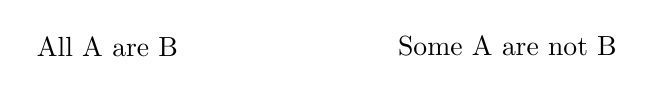
\begin{tikzpicture}
        \draw (0,1.25) node {All A are B};
        \allXareY{A}{B}
        \begin{scope}[shift={(2in,0in)}]
        \draw (0,1.25) node {Some A are not B};
        \someXarenotY{A}{B}
        \end{scope}
      \end{tikzpicture}
  
    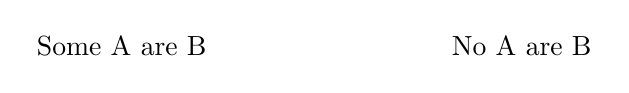
\begin{tikzpicture}
        \draw (0,1.25) node {Some A are B};
        \someXareY{A}{B}
        \begin{scope}[shift={(2in,0in)}]
        \draw (0,1.25) node {No A are B};
        \noXareY{A}{B}
        \end{scope}
      \end{tikzpicture}  
         
    True $\longleftarrow$ False
    \end{center} 
    
\end{frame}

\begin{frame}
  \frametitle{Existential fallacy}
  
  \begin{block}{A good argument?}
    \begin{itemize}
      \item No A are B
      \item $\therefore$, it is false that all A are B
    \end{itemize}
  \end{block}
  
  \uncover<2->{
  \begin{tikzpicture}
    \draw (0,1.25) node {No A are B};
    \noXareY{A}{B}
    \begin{scope}[shift={(0in,-1in)}]
      \draw (0,1.25) node {All A are B};
      \allXareY{A}{B}
      \draw[->] (3,0) -- (3.5,0);
      \uncover<3->{\draw[->] (3,1.5) -- (3.5,1) node[pos=.5] {$|$};} 
        \begin{scope}[shift={(2in,0in)}]
          \draw (0,1.25) node {Some A are not B};
          \someXarenotY{A}{B}
        \end{scope}
    \end{scope}
  \end{tikzpicture}
  }
\end{frame}

\subsection{Structural}

\frame{
\frametitle{Conversion}
\framesubtitle{Structural relation}

\begin{block}{Switch the subject and predicate terms}
\begin{center}
  [Quantifier] A [copula] B $\longrightarrow$ [Quantifier] B [copula] A
\end{center}
\end{block}

\begin{block}<2->{Be careful!} 
  \begin{itemize}
    \item Conversion is a \textit{syntactic} relation between propositions.
    \item Conversion does not necessarily preserve truth.
    \item $No$ and $Some$ propositions are equivalent to their conversions.
    \item $All$ and $Some-not$ propositions are not equivalent to their conversions. (illicit conversion)
  \end{itemize}
\end{block}
}

\frame{
\frametitle{Conversion}
\framesubtitle{Example}

\begin{block}{Equivalent}
No $A$ are $B$ $\longrightarrow$ No $B$ are $A$
\end{block}

\begin{center}
\begin{tikzpicture}
  \noXareY{A}{B}
  \draw[->] (1.1in,0in) -- (1.5in,0in);
  \begin{scope}[shift={(2in,0in)}]
    \noXareY{B}{A}
  \end{scope}
\end{tikzpicture}
\end{center}

\begin{block}{Not equivalent}
All $A$ are $B$ $\longrightarrow$ All $B$ are $A$
\end{block}
\begin{center}

\begin{tikzpicture}
  \allXareY{A}{B}
  \draw[->] (1.1in,0in) -- (1.5in,0in);
  \begin{scope}[shift={(2in,0in)}]
    \allXareY{B}{A}
  \end{scope}
\end{tikzpicture}
\end{center}

}

\frame{
\frametitle{Obversion}
\framesubtitle{Structural relation}

\begin{block}{Flip and negate the predicate term}
  \begin{itemize}
    \item First, flip the \textit{quality} of the proposition.
    \begin{itemize}
      \item $All \longleftrightarrow No$
      \item $Some \longleftrightarrow Some-not$
    \end{itemize}
    \item Second, take the \textit{class complement} of the predicate term. ($B \longrightarrow non-B$)
      \begin{itemize}
        \item The complement of a class is everything that is not a member of that class.
        \item In a Venn diagram, the class complement is \textit{all the space outside} of the circle representing the class.
      \end{itemize}
  \end{itemize}
\end{block}

\begin{block}<2->{Have no fear!}
  \begin{itemize}
    \item Obversion is also a syntactic relation.
    \item But it is one that preserves truth in all instances.
    \item So, categorical propositions are \textit{equivalent} to their obverses.
  \end{itemize}
\end{block}
}

\frame{
\frametitle{Obversion}
\framesubtitle{Example}

\begin{block}{Equivalent}
  Some $A$ are $B$ $\longrightarrow$ Some $A$ are not $non-B$
\end{block}

\begin{center}
\begin{tikzpicture}
  \someXareY{A}{B}
  \draw[->] (1.1in,0in) -- (1.5in,0in);
  \begin{scope}[shift={(2in,0in)}]
    \someXareY{A}{B}
  \end{scope}
\end{tikzpicture}
\end{center}

}

\frame{
\frametitle{Contraposition}
\framesubtitle{Structural relation}

\begin{block}{Switch and negate both terms}
  \begin{itemize}
    \item First, switch the subject and predicate term (just like conversion).
    \item Next, take the class complement of both the terms.
    \item $\;$ [Quantifier] A [copula] B $\longrightarrow$ [Quantifier] $non-$B [copula] $non-$A
  \end{itemize}
\end{block}

\begin{block}<2->{Watch out!}
  \begin{itemize}
    \item Like conversion, contraposition is not universally valid.
    \item $All$ and $Some-not$ propositions are equivalent to their conversions.
    \item $No$ and $Some$ propositions are not equivalent to their conversions. (illicit conversion)
  \end{itemize}
\end{block}
}

\frame{
\frametitle{Contraposition}
\framesubtitle{Example}

\begin{block}{Equivalent}
All $A$ are $B$ $\longrightarrow$ All $non-B$ are $non-A$
\end{block}

\begin{center}
\begin{tikzpicture}
  \allXareY{A}{B}
  \draw[->] (1.1in,0in) -- (1.5in,0in);
  \begin{scope}[shift={(2in,0in)}]
    \allYareX{B}{A}
  \end{scope}
\end{tikzpicture}
\end{center}

\begin{block}{Not equivalent}
Some $A$ are $B$ $\longrightarrow$ Some $non-B$ are $non-A$
\end{block}
\begin{center}

\begin{tikzpicture}
  \someXareY{A}{B}
  \draw[->] (1.1in,0in) -- (1.5in,0in);
  \begin{scope}[shift={(2in,0in)}]
      \draw \firstcircle node [below left=.25in] {B};
      \draw \secondcircle node [below right=.25in] {A};
      \node [above right=.25in] (x2) {x};
  \end{scope}
\end{tikzpicture}
\end{center}

}
\end{document}
